% generated by scripts/pkl_to_latex.py
% source PKL : thermal_v1_L8_Ne8_U10_t1_mode-uniform_tpall_t2all_tperpall_nmin2_solver-gcg_full_restarts8_iter200_kmax4_tol1em09_cut10_adaptive1_step5_clusteravg1_T0to0.5_N20-3c87501b406b_knone_diag0.pkl
% scan type  : Tscan
% state      : gs
% quantity   : purity
% x-max cap  : 0.5
% requires   : \usepackage{pgfplots} \pgfplotsset{compat=1.18}
% colours match the matplotlib PDF (tab10 cycle)
\definecolor{gmeC0}{HTML}{1F77B4}
\definecolor{gmeC1}{HTML}{FF7F0E}
\definecolor{gmeC2}{HTML}{2CA02C}
\definecolor{gmeC3}{HTML}{D62728}
\definecolor{gmeC4}{HTML}{9467BD}
\definecolor{gmeC5}{HTML}{8C564B}
\definecolor{gmeC6}{HTML}{E377C2}
\definecolor{gmeC7}{HTML}{17BECF}

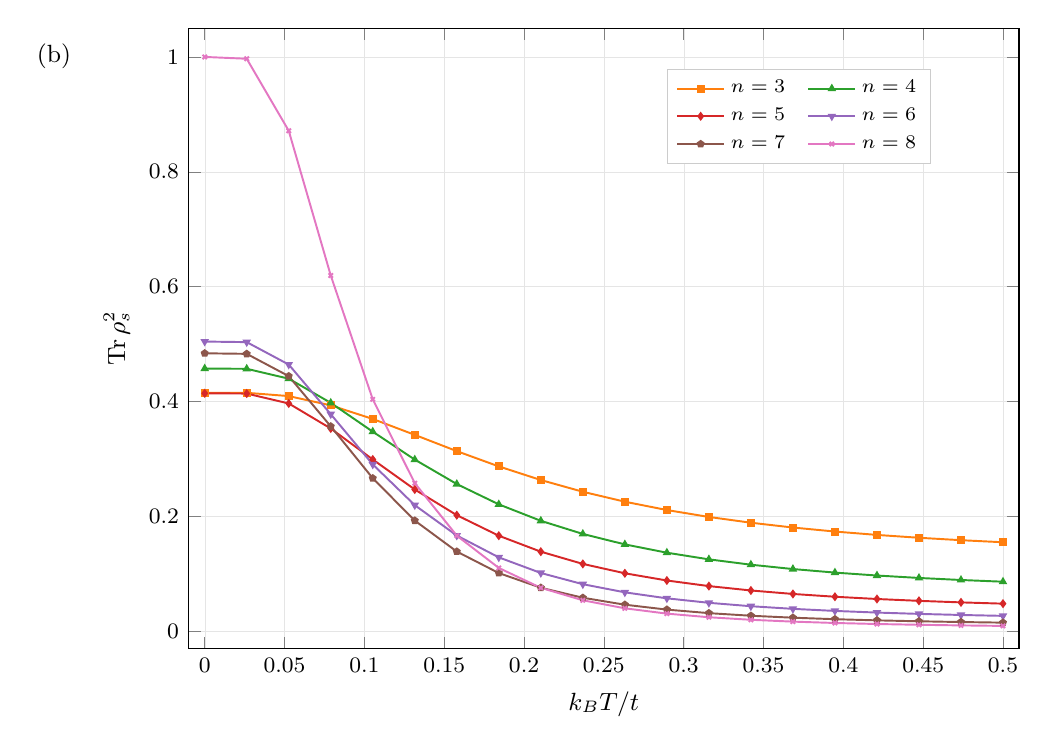
\begin{tikzpicture}
  \begin{axis}[
    width=\columnwidth,
    height=0.78\columnwidth,
    xlabel={$k_B T/t$},
    ylabel={$\mathrm{Tr}\,\rho_s^2$},
    grid=both,
    grid style={line width=.1pt, draw=gray!20},
    tick label style={font=\footnotesize\rmfamily, /pgf/number format/fixed},
    label style={font=\small\rmfamily},
    scaled ticks=false,
    legend style={font=\scriptsize\rmfamily, draw=gray!40, at={(0.5,1.03)}, anchor=south, /tikz/every even column/.append style={column sep=6pt}},
    legend cell align={left},
    legend columns=2,
    ymin=-0.03,
    ymax=1.05,
    xmin=-0.01,
    xmax=0.51,
    legend style={at={(0.735,0.858)}, anchor=center, fill=white},
    after end axis/.append code={\node[anchor=east, font=\small\rmfamily] at (axis description cs:-0.13,0.954) {(b)};},
  ]
    \addplot[color=gmeC1, mark=square*, mark size=1.1pt, line width=0.7pt] coordinates {
        (0,0.415247) (0.026316,0.415114) (0.052632,0.409375) (0.078947,0.393257)
        (0.105263,0.369567) (0.131579,0.341849) (0.157895,0.313529) (0.184211,0.286931)
        (0.210526,0.263221) (0.236842,0.242762) (0.263158,0.225451) (0.289474,0.210963)
        (0.315789,0.198899) (0.342105,0.188861) (0.368421,0.180495) (0.394737,0.173498)
        (0.421053,0.167619) (0.447368,0.162655) (0.473684,0.158439) (0.5,0.154841)
    };
    \addlegendentry{$n=3$}
    \addplot[color=gmeC2, mark=triangle*, mark size=1.1pt, line width=0.7pt] coordinates {
        (0,0.457304) (0.026316,0.456891) (0.052632,0.439691) (0.078947,0.397635)
        (0.105263,0.347386) (0.131579,0.298786) (0.157895,0.256207) (0.184211,0.220812)
        (0.210526,0.192179) (0.236842,0.169312) (0.263158,0.151127) (0.289474,0.136649)
        (0.315789,0.125071) (0.342105,0.115751) (0.368421,0.108192) (0.394737,0.102011)
        (0.421053,0.096914) (0.447368,0.092678) (0.473684,0.089129) (0.5,0.086134)
    };
    \addlegendentry{$n=4$}
    \addplot[color=gmeC3, mark=diamond*, mark size=1.1pt, line width=0.7pt] coordinates {
        (0,0.414191) (0.026316,0.413782) (0.052632,0.396564) (0.078947,0.352934)
        (0.105263,0.299001) (0.131579,0.246718) (0.157895,0.202011) (0.184211,0.166213)
        (0.210526,0.138429) (0.236842,0.117124) (0.263158,0.100808) (0.289474,0.088252)
        (0.315789,0.078507) (0.342105,0.070867) (0.368421,0.06481) (0.394737,0.059955)
        (0.421053,0.056021) (0.447368,0.052799) (0.473684,0.050135) (0.5,0.047912)
    };
    \addlegendentry{$n=5$}
    \addplot[color=gmeC4, mark=triangle*, mark size=1.1pt, mark options={rotate=180}, line width=0.7pt] coordinates {
        (0,0.504323) (0.026316,0.50336) (0.052632,0.464313) (0.078947,0.377842)
        (0.105263,0.290348) (0.131579,0.219411) (0.157895,0.166568) (0.184211,0.128508)
        (0.210526,0.10132) (0.236842,0.081804) (0.263158,0.067635) (0.289474,0.057199)
        (0.315789,0.049389) (0.342105,0.043449) (0.368421,0.038859) (0.394737,0.035259)
        (0.421053,0.032396) (0.447368,0.030088) (0.473684,0.028206) (0.5,0.026654)
    };
    \addlegendentry{$n=6$}
    \addplot[color=gmeC5, mark=pentagon*, mark size=1.1pt, line width=0.7pt] coordinates {
        (0,0.483894) (0.026316,0.482941) (0.052632,0.444109) (0.078947,0.35669)
        (0.105263,0.266317) (0.131579,0.1926) (0.157895,0.138654) (0.184211,0.101197)
        (0.210526,0.075656) (0.236842,0.058197) (0.263158,0.046101) (0.289474,0.03756)
        (0.315789,0.031402) (0.342105,0.026868) (0.368421,0.023461) (0.394737,0.020852)
        (0.421053,0.018819) (0.447368,0.01721) (0.473684,0.015918) (0.5,0.014866)
    };
    \addlegendentry{$n=7$}
    \addplot[color=gmeC6, mark=x, mark size=1.1pt, line width=0.7pt] coordinates {
        (0,1) (0.026316,0.996827) (0.052632,0.871422) (0.078947,0.619397)
        (0.105263,0.403705) (0.131579,0.257848) (0.157895,0.166305) (0.184211,0.11011)
        (0.210526,0.075493) (0.236842,0.053782) (0.263158,0.039813) (0.289474,0.030559)
        (0.315789,0.024246) (0.342105,0.019815) (0.368421,0.01662) (0.394737,0.01426)
        (0.421053,0.012477) (0.447368,0.011104) (0.473684,0.010026) (0.5,0.009168)
    };
    \addlegendentry{$n=8$}
  \end{axis}
\end{tikzpicture}
